% This is samplepaper.tex, a sample chapter demonstrating the
% LLNCS macro package for Springer Computer Science proceedings;
% Version 2.20 of 2017/10/04
%
\documentclass[runningheads]{llncs}
%
\usepackage{graphicx}
\usepackage{csquotes}
\usepackage{hyperref}
\usepackage{listings}

% Used for displaying a sample figure. If possible, figure files should
% be included in EPS format.
%
% If you use the hyperref package, please uncomment the following line
% to display URLs in blue roman font according to Springer's eBook style:
% \renewcommand\UrlFont{\color{blue}\rmfamily}

\begin{document}
%
\title{Evolution of the Spineless Tagless G-Machine}
%
%\titlerunning{Spineless Tagless G-Machine}
% If the paper title is too long for the running head, you can set
% an abbreviated paper title here
%
\author{Armin Bernstetter}
%
\authorrunning{Armin Bernstetter}
% First names are abbreviated in the running head.
% If there are more than two authors, 'et al.' is used.
%
\institute{Seminar Funktionale Programmierung \\ Julius-Maximilians-Universität, Würzburg}
%\institute{Princeton University, Princeton NJ 08544, USA \and
%Springer Heidelberg, Tiergartenstr. 17, 69121 Heidelberg, Germany
%\email{lncs@springer.com}\\
%\url{http://www.springer.com/gp/computer-science/lncs} \and
%ABC Institute, Rupert-Karls-University Heidelberg, Heidelberg, Germany\\
%\email{\{abc,lncs\}@uni-heidelberg.de}}
%
\maketitle              % typeset the header of the contribution
%
\begin{abstract}
The spineless tagless G-machine (STGM) is an abstract machine that is located at the core of the Glasgow Haskell Compiler GHC. Since its creation at the start of Haskell development in early 1990s it has undergone several significant changes. This work aims at showing the evolution of the STGM and overall at providing insight in the workings of the most widely-used Haskell compiler GHC.

%\keywords{First keyword  \and Second keyword \and Another keyword.}
\end{abstract}
%
%
%

\section{Introduction}

This work provides an insight in the compilation process of the lazy, purely functional programming language Haskell. For this we take a look inside the Glasgow Haskell Compiler, today the most used compiler for Haskell [citation needed]. Located at its core is the \textit{Spineless Tagless G-Machine}, an abstract machine used as a bridge between high level code and machine code.

Described in detail in the 1992 paper \textit{Implementing Lazy functional languages on stock hardware: the Spineless Tagless G-machine} \cite{jones1992implementing}, the STGM has undergone several significant changes since then. Two papers highlighting these changes are \textit{Making a Fast Curry: Push/Enter vs.
Eval/Apply for Higher-order Languages}\cite{marlow2004making} and \textit{Faster Laziness Using Dynamic Pointer Tagging}\cite{marlow2007faster}. The former introducing the switch from the \textit{push/enter} evaluation method to the \textit{eval/apply} (see section BLA), the latter introducing dynamic pointer tagging which revokes the \enquote{tagless} part in the name of the STGM.

Section \ref{sec:basics} provides basic information about Haskell and compilers in general.

Section \ref{sec:ghc} describes GHC, the \textit{Glasgow Haskell Compiler} which is the most widely-used Haskell compiler. This section introduces the building blocks that GHC consists of.

Section \ref{sec:stgm} takes a more in-depth look into the \textit{Spineless Tagless G-Machine}, an abstract machine that stands between Haskell code and assembly code in GHC's compilation process.

Section \ref{sec:conclusion} concludes with a retrospective overview of STGM and its changes throughout the last 30 years.


\newpage
\section{Basics}
\label{sec:basics}

This section introduces basics about compilers, Haskell and functional programming in general.

\subsection{Haskell}
Haskell is a purely functional programming language that emerged during the late 1980s and early 1990s. It was created with the goal of finding a common functional language to improve interactivity and exchange between programmers and researchers since, at the time, many lesser known functional programming languages existed. A committee consisting of Paul Hudak, John Hughes, Simon Peyton Jones, Philip Wadler and others was created and met several times until in 1990 the Haskell 1.0 Report was published \cite{hudak2007history}.

\subsection{Compilers}
A compiler is a software system consisting of several phases, that translates programs from a higher-level language to machine code. \cite{muchnick1997advanced}

In general, these phases are \textit{lexical analysis}, \textit{syntactic analysis or parsing}, \textit{semantic checking} and \textit{code generation}. \cite{muchnick1997advanced}

\begin{figure}

\centering
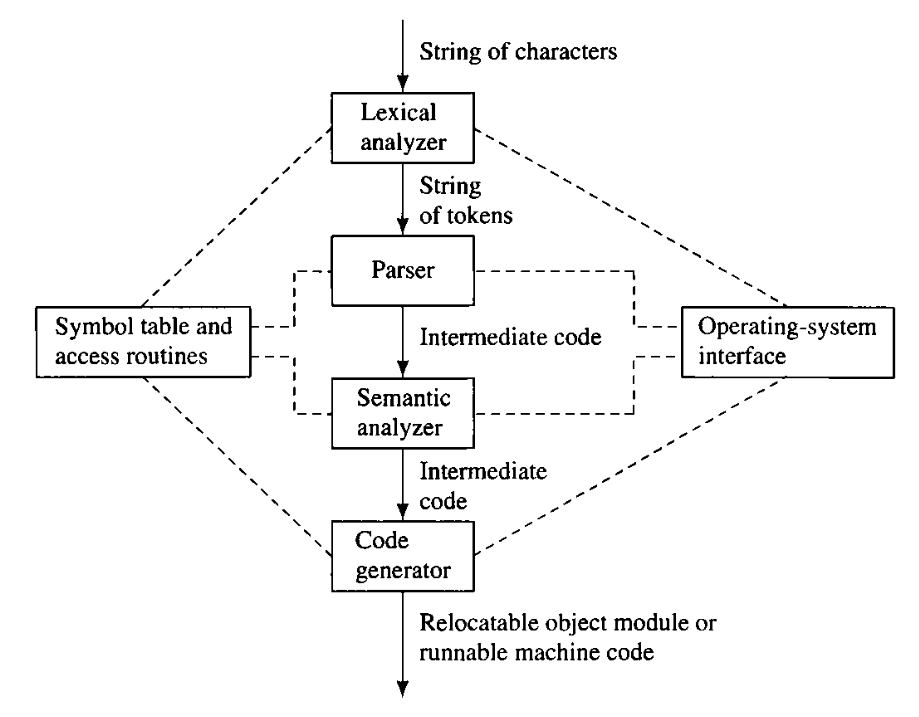
\includegraphics[width=10cm]{compiler.png}
\caption{General illustration of the phases of a compiler taken from Muchnik \cite{muchnick1997advanced}.}
\label{fig:compiler}
\end{figure}

\paragraph{Lexical Analysis} analyzes the character string and produces errors in case any part of the program string is not parseable into legal tokens. Legal in this case refers to tokens that are members of the vocabulary of the respective programming language.

\paragraph{Syntactic Analysis/Parsing} parses the program into an intermediate representation. An example would be a parse tree accompanied by a symbol table containing information on identifiers used in the program and their attributes. This phase may also produce error messages if syntax errors are detected.

\paragraph{Semantic Checking} examines the program for static-semantic validity. This phase takes as input the intermediate representation and determines whether the program satisfies the requirements for the static-semantic properties of the source language.

\paragraph{Code Generation} finally transforms the intermediate representation into machine code which can then be executed. 


These phases are often complemented by additional steps in many compilers, the Glasgow Haskell Compiler being one of those (see Section \ref{sec:ghc}).

\subsection{Abstract Machines}
This section describes the concept of abstract machines. They bridge the gap between high level source code and machine code by providing an intermediate language stage for compilation. Abstract machines are located in the space between the two extremes of being a small intermediate language and being a model for a real machine that is yet to be built \cite{diehl2000abstract}.

Abstract machines execute programs step-by-step in a loop. This execution loop iterates over a sequence of instructions often using a stack and register with the program counter as a special register pointing at the next instruction. \cite{diehl2000abstract}

Abstract machines introduce an additional layer of abstraction to the implementation of compilers for programming languages.

Examples for such abstract machines or related concepts are the Java Virtual Machine and the Spineless Tagless G-Machine which is the focus of this work.

\section{GHC}
\label{sec:ghc}

\href{https://downloads.haskell.org/~ghc/7.8.1/docs/html/users_guide/an-external-representation-for-the-ghc-core-language-for-ghc-6.10.html}{link ghc 7.8.1}

\href{https://downloads.haskell.org/ghc/8.6.5/docs/html/users_guide}{link ghc 8.6.5}

The Glasgow Haskell Compiler, named after the city where its development began, is the most widely-used Haskell compiler \cite{marlow2007faster}. It is the de facto default compiler for Haskell and is shipped with the \textit{Haskell Platform} downloadable at \url{https://www.haskell.org/}.

Figure \ref{fig:ghc} illustrates the different phases program code is passed through during compilation. In contrast to the general compiler structure shown in figure \ref{fig:compiler}, GHC has several additional intermediate steps. The Haskell source code is initially parsed and translated to a reduced \textit{Core} language which is then again translated to the \textit{STG representation}. A code generator (the \textit{STGM}) generates \texttt{C--} code followed by three possible paths for finally generating machine code.

\begin{figure}

\centering
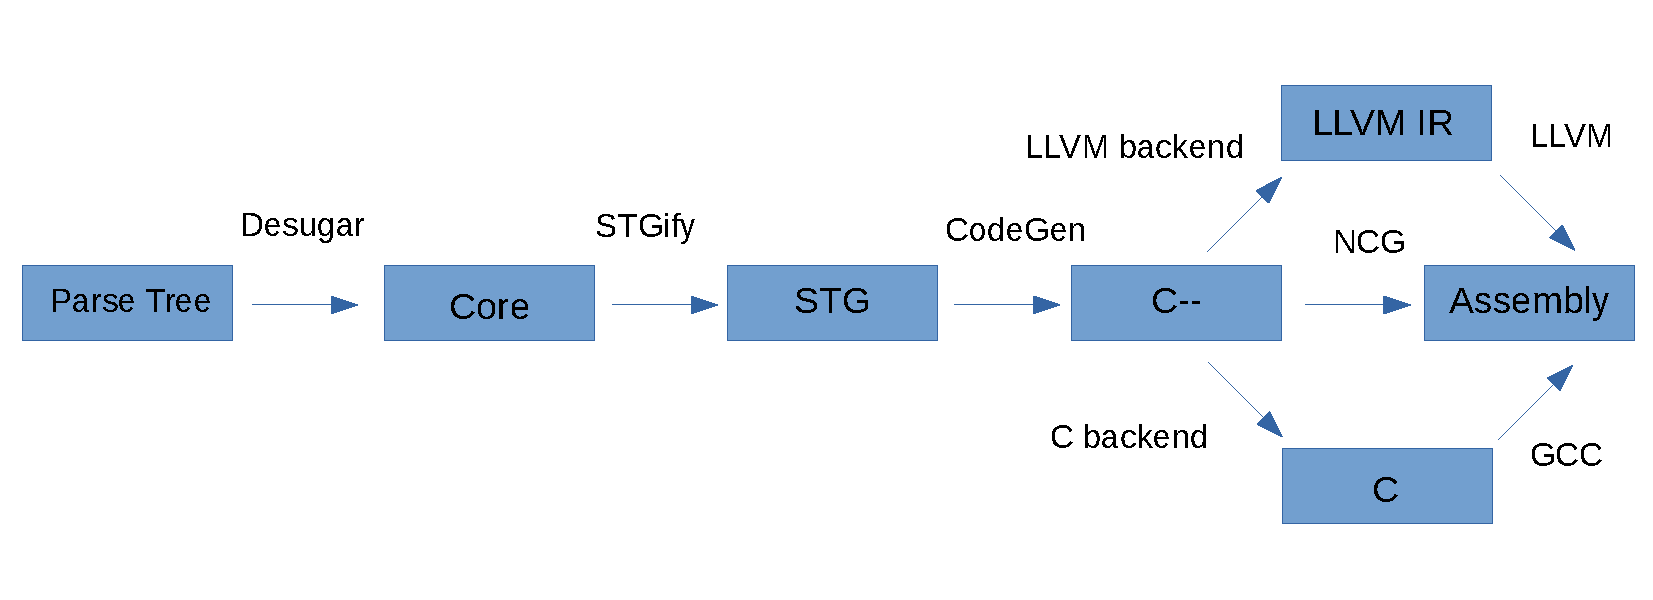
\includegraphics[width=12cm]{ghcflow.pdf}
\caption{GHC's compilation phases. Own graphic based on a depiction from the official GHC gitlab repository \protect\footnotemark}
\label{fig:ghc}
\end{figure}
\footnotetext{\url{https://gitlab.haskell.org/ghc/ghc/wikis/commentary/compiler/generated-code}}

\subsection{Core Language}
The core language is a variant of Haskell in where all syntactic sugar is removed and resolved e.g. the do-notation or type aliases. It consists of Haskell's central data types and is a small, explicitly-typed variant of the typed lambda calculus System F \cite{girard1986system} which is called System FC \cite{sulzmann2007system}. Type checking is performed here, overloading is resolved and pattern-matching is translated into \texttt{case} expressions where each one performs only a single level of matching \cite{jones1992implementing}.

\subsection{The STGM Language}
The core language is then translated to the \textit{STG Language}.
This language is a purely functional programming language on its own that is used as an intermediate representation.

syntax details?

heap object layouts?


Move to "in depth" section?

\subsection{\texttt{C--}}

A code generator (the STG machine) translates the STG language into \texttt{C--}.

\texttt{C--} is a programming language developed by Simon Peyton-Jones as a portable backend-language for compilers. Where C++ can be seen as an extension of the C language, \texttt{C--} is to be thought of as a reduction to a smaller core language. \texttt{C--} in general is made for being generated by compilers and not for being written by programmers. \cite{jones1999c}

paragraph



\paragraph{Why is it needed? C and Stack stuff?}


\subsection{Backends}
GHC supports the generation of assembly machine code via several backends.


\subsubsection{C Backend}
The C backend uses the \textit{GNU Compiler Collection} GCC but is deprecated

\subsubsection{Native Code Generator}
The Native Code Generator is the default way used in GHC.

\subsubsection{LLVM}
LLVM is a modern portable compiler framework that was developed as an alternative to the classic GCC toolchain. Its acronym stands for \textit{Low Level Virtual Machine} \cite{lattner2004llvm}

Using LLVM in GHC results in similar compilation performance as the NCG but can lead to faster performing executables.

\section{STGM in depth}
\label{sec:stgm}

The Spineless Tagless G-Machine is an abstract machine for non-strict functional languages.
It was developed by Simon Peyton Jones as an alternative or successor to other such abstract machines like the \textit{Three Instruction Machine (TIM)} by Fairbairn and Wray \cite{fairbairn1987tim} and the \textit{G-Machine} by Johnsson \cite{johnsson1984efficient}.

Vielleicht zuerst einfach nur den Status von 1992 zeigen und dann die Änderungen? (Push/enter $->$ eval/apply und tagless $->$ dynamic pointer tagging)
-> Sehr gute Idee!

\cite{jones1992implementing}

\subsubsection{Graph reducing}

\subsubsection{Spineless}
Spineless refers to the way the code is represented on the machine.

STG programs are not represented as a tree but as a graph. Therefore, in memory a STG program is not a contiguous block of memory but smaller parts of the graph that reference each other.

\subsubsection{Tagless}

\textbf{SPJONES 1993 Seite 12}

\textbf{SPJONES 1993 Seite 5}
The term tagless refers to the way the STG-machine evaluates a heap closure. 


[EVERYTHING FROM THE INTRODUCTION OF THE POINTER TAGGING PAPER]


\subsection{Function application}
\textbf{in SPjones 1993 Seite 14/15}

Function calls in a lazy functional languages with currying and partial application require special mechanisms in compilers.
\enquote{Currying} is one of the core principles of lazy functional languages 

[INSERT DETAILS ABOUT CURRYING]


HOW TO INCLUDE THE EVALUATION TRACE?



\subsubsection{Push/Enter}


\subsection{Changes}

\subsubsection{Eval/Apply}

\subsubsection{Dynamic Pointer Tagging}
In 2007, Marlow et al.\cite{marlow2007faster} found that Haskell programs compiled by GHC show mispredicted branches on modern processors. This led to a re-examination of the \enquote{tagless} aspect of the STGM. The result were significant performance improvements.


\section{Conclusion}
\label{sec:conclusion}

This work 


% ---- Bibliography ----
%
% BibTeX users should specify bibliography style 'splncs04'.
% References will then be sorted and formatted in the correct style.
%
\newpage
\bibliographystyle{splncs04}
\bibliography{stgm.bib}
\end{document}
